%% LyX 2.3.6 created this file.  For more info, see http://www.lyx.org/.
%% Do not edit unless you really know what you are doing.
\documentclass[english]{achemso}
\usepackage[T2A,LGR,T1]{fontenc}
\usepackage{babel}
\usepackage{array}
\usepackage{textcomp}
\usepackage{url}
\usepackage{multirow}
\usepackage{amsmath}
\usepackage{graphicx}
\usepackage{subscript}
\usepackage[unicode=true,pdfusetitle,
 bookmarks=true,bookmarksnumbered=false,bookmarksopen=false,
 breaklinks=false,pdfborder={0 0 0},pdfborderstyle={},backref=false,colorlinks=false]
 {hyperref}

\makeatletter

%%%%%%%%%%%%%%%%%%%%%%%%%%%%%% LyX specific LaTeX commands.


\title{Wetting of adhesive fluid controls insect adhesion in air and underwater}


\author{Pranav Sudersan}


\affiliation{Max Planck Institute for Polymer Research, Ackermannweg 10, 55128
Mainz, Germany}


\author{Michael Kappl}


\affiliation{Max Planck Institute for Polymer Research, Ackermannweg 10, 55128
Mainz, Germany}


\author{Thomas Endlein}


\affiliation{Max Planck Institute for Polymer Research, Ackermannweg 10, 55128
Mainz, Germany}


\author{Bat-El Pinchasik}


\affiliation{School of Mechanical Engineering, Tel Aviv University, Tel Aviv-Yafo,
Israel}


\author{Hans-J\"{u}rgen Butt}


\affiliation{Max Planck Institute for Polymer Research, Ackermannweg 10, 55128
Mainz, Germany}


\email{butt@mpip-mainz.mpg.de}


\phone{+49 6131 379 111}


\fax{+49 6131 379 310}

\DeclareRobustCommand{\greektext}{%
  \fontencoding{LGR}\selectfont\def\encodingdefault{LGR}}
\DeclareRobustCommand{\textgreek}[1]{\leavevmode{\greektext #1}}
\ProvideTextCommand{\~}{LGR}[1]{\char126#1}

\DeclareRobustCommand{\cyrtext}{%
  \fontencoding{T2A}\selectfont\def\encodingdefault{T2A}}
\DeclareRobustCommand{\textcyr}[1]{\leavevmode{\cyrtext #1}}

\newcommand{\lyxmathsym}[1]{\ifmmode\begingroup\def\b@ld{bold}
  \text{\ifx\math@version\b@ld\bfseries\fi#1}\endgroup\else#1\fi}

%% Because html converters don't know tabularnewline
\providecommand{\tabularnewline}{\\}

%%%%%%%%%%%%%%%%%%%%%%%%%%%%%% User specified LaTeX commands.
\SectionNumbersOn
%\setkeys{acs}{doi = true}
\setkeys{Gin}{width=\linewidth}
\usepackage{subcaption}

\makeatother

\begin{document}
\begin{abstract}
Insects like beetles can stick to various surfaces using hairy pads
mediated by an oily adhesive fluid. It was previously shown that the
pads can even attach underwater, presumably due to an air bubble trapped
around the pad. However, the bubble's relative contribution to adhesion
via capillary force remains unclear. To investigate the exact role
of bubble, in this study, we perform\emph{ in-vivo} underwater adhesion
measurements of a ladybug's pad, in the presence and absence of the
trapped bubble and compare it with its adhesion in air. Our experiments
reveal that on a hydrophobic substrate, even without a bubble, the
pad can show adhesion underwater comparable to that in air. On a hydrophilic
substrate, underwater adhesion is significantly reduced, with or without
a trapped bubble. To explain these results, we develop a simple theoretical
model to estimate the net adhesion of a hairy pad due to capillary
forces. Our results demonstrate that the wetting properties of the
adhesive fluid determines the insect's adhesion in both air and underwater
conditions.
\end{abstract}

\section{Introduction}

The question of how insects can walk on smooth surfaces against gravity
has fascinated scientists for at least the past three centuries \cite{RN198,RN59}.
We now know that such animals are able to adhere by using specialized
organs on their feet called adhesive pads. These adhesive pads exist
in a variety of types depending on the animal, but are generally categorized
into: 1) ``smooth pads'' found in ants\cite{RN201}, stick insects
\cite{RN182}, etc. and 2) ``hairy pads'' seen in flies \cite{RN155},
geckos \cite{RN202} and others. The hairy pads show: 1) compliance
to rough surfaces due to their lower effective modulus, 2) angle dependent
adhesion due to asymmetric hair geometry and 3) self-cleaning capability
\cite{RN20}, which makes them suitable to adhere to most surfaces
reversibly. Many of these insects pads also secrete an adhesive fluid,
as seen in flies and ants \cite{RN201} (``wet adhesion''), while
others such as spiders and geckos rely on their dry hairy pads for
attachment (``dry adhesion''). In the ``wet adhesion'' case, fluid
secretion can enforce adhesion through surface tension and viscous
forces \cite{RN71}, while, ``dry adhesion'' relies mostly on van
der Waals forces \cite{RN202}. 

Terrestrial beetles such as the dock beetle or the ladybug have hairy
pads consisting of a dense array of hair-like structures called setae.
The setae tips can be discoidal, spatula or pointed shaped, which
are distributed throughout the pad depending on sex or species\cite{RN19}.
Single seta force measurements revealed that discoidal shaped seta
shows larger pull-off force than spatula and pointed setae\cite{RN79},
illustrating the role of hair geometry in adhesion. The tip of each
seta secretes approximately one femtoliter of oily adhesive fluid
\cite{RN108}. The fluid's chemical composition is identified as a
mixture of mostly long chain hydrocarbons\cite{RN96} with traces
of triglycerides, fatty acids and cholesterol\cite{RN221,RN222}.
A recent study by Gernay et. al.\cite{RN77}, based on an elastocapillary
model, has been able to reasonably predict single seta adhesion forces
theoretically, confirming the dominant role of surface tension in
the ``wet adhesion'' of beetles.

While most of the studies on insect adhesion are done under natural
conditions in air, insect attachment underwater has been relatively
unexplored. Typically, underwater adhesion is complicated to achieve
due to the difficulty in displacing the water layer and enable good
contact\cite{RN123}. Regardless, a study on leaf beetles\cite{RN87}
has revealed that they can in fact attach quite well to surfaces underwater.
Its hairy pad traps an air bubble underwater, which dewets the surface
on contact. It has been hypothesized that a combination of capillary
forces due the air bubble and hair contact within the dewetted area
results in its adhesion underwater. However, a detailed investigation
of the bubble's contribution and necessity to adhere to different
surfaces is lacking. Geckos are also known to adhere underwater, where
its shear adhesion force on hydrophobic substrates are similar in
both air and underwater conditions. Interestingly, its adhesion on
a fluorinated substrate is even larger underwater than in air\cite{RN15}.
This has been partially explained by a thermodynamic work of adhesion
model, assuming full displacement of water at the interface, leading
to a dry ``van der Waals'' contact of hairs with the surface\cite{RN199}.

The goal of this paper is to provide a generalized picture of adhesion
in insects which use hairy pads secreting a fluid for attachment.
First, we perform adhesion measurements of a single constrained pad
of a live ladybug beetle in air and underwater conditions, both on
smooth hydrophilic and hydrophobic glass surfaces, with a microscopic
observation of the contact process. Second, we develop a simple theoretical
model considering capillary forces to predict the net adhesion force
of a hairy pad under different conditions. Finally, we discuss key
insights gained from our experiments and model, as well as possible
implications in understanding adhesion in other animals.

\section{Experimental}

Normal adhesion force measurements on a restrained leg of a live ladybug
beetle were performed. We characterize adhesion by the pull-off force
during detachment. Measurements were done against smooth glass and
fluorinated surfaces to represent hydrophilic and hydrophobic substrates
respectively. When no water was present, we labeled the contact type
as ``\emph{in air}''. For the underwater conditions, measurements
were done both in the presence and absence of a trapped bubble (``\emph{underwater:
bubble}'' and ``\emph{underwater: no bubble}'', respectively) to
investigate the bubble's role in underwater adhesion. Adhesion force
for each of the labeled contact types were compared for both substrates.

\subsection{Material and Methods}

\subsubsection{Insect preparation}

Seven-spotted adult ladybug beetles (\emph{Coccinella septempuctata})
purchased from Katz Biotech (Baruth, Germany) were used for adhesion
tests. The beetles were housed in a plastic box filled with leaves,
twigs and stones at room temperature and 60-80\% relative humidity
with daily access to sunlight. They were fed with raisins, honey and
water\emph{ ad libitum}. 

Experiments were done on male beetles. Each leg of the beetle has
a pair of hairy pads covered with mostly discoidal shaped setae, capable
of strong adhesion. For the test, we only allowed the distal-end pad
to make contact. The beetle's leg was constrained similar to the method
described by Bullock et al \cite{RN19}. A steel ball fixed with a
piece of thick solder wire served as a rotatable holder to fix the
beetle and align its leg (Figure \ref{fig:Setup}). The beetle was
first anesthetized using CO\textsubscript{2} sublimating from a piece
of dry ice and then glued to the steel ball on its back. Its front
left leg was carefully fixed to the solder wire of the holder using
Blue-Tac. Its claws were fixed using epoxy glue to prevent any wiggling.
A small piece of non-sticky Teflon tape helped to keep its other legs
tucked close to the body and avoid their interference during the adhesion
test.

After measurements, the beetle was freed by carefully removing the
epoxy glue and Blue-Tac without harming it and set free.

\subsubsection{Substrate preparation}

Standard 20 mm wide glass coverslips were used as the hydrophilic
substrate. Glass was wiped with isopropanol, rinsed in water and dried
under nitrogen flow. The surface was then plasma cleaned in a oxygen
plasma chamber (Diener Electronic Femto) for 10 min at 120 W. The
surface was further rinsed with water and dried under nitrogen flow.

For the hydrophobic substrate, the glass cover slip was coated with
a fluorosilane via chemical vapor deposition (CVD). First, the glass
was cleaned using IPA and plasma treated as before. Next, 0.2 ml of
Trichloro(1H,1H,2H,2H-perfluorooctyl) silane (PFOTS), procured from
Sigma Aldrich, was put in a sealed chamber along with the the cleaned
glass. The chamber was placed under 100 mbar pressure for 10 min for
the CVD process. Finally, the substrate was annealed at 150\textcelsius{}
for 3 hours.

The substrate wettability was characterized by dynamic contact angle
measurements, performed with a DataPhysics OCA 35 contact angle goniometer.
De-ionized water and n-hexadecane were used as test liquids. Advancing
and receding contact angles were measured for a maximum drop volume
of 10 \textgreek{m}l and with 0.5 \textgreek{m}l/s flow rate. Static
contact angles were measured for a 5 \textgreek{m}l drop.

\begin{table}[H]
\centering{}%
\begin{tabular}{|c|c|c|c|c|}
\hline 
Substrate & Liquid & \ensuremath{\theta}\textsubscript{A} & \ensuremath{\theta}\textsubscript{R} & \ensuremath{\theta}\textsubscript{S}\tabularnewline
\hline 
\hline 
\multirow{2}{*}{Glass} & Water & 63\ensuremath{\pm}5\textdegree{} & 20\ensuremath{\pm}2\textdegree{} & 57\ensuremath{\pm}2\textdegree{}\tabularnewline
\cline{2-5} \cline{3-5} \cline{4-5} \cline{5-5} 
 & n-Hexadecane & <10\textdegree{} & <10\textdegree{} & <10\textdegree{}\tabularnewline
\hline 
\multirow{2}{*}{PFOTS} & Water & 122\ensuremath{\pm}1\textdegree{} & 93\ensuremath{\pm}2\textdegree{} & 110\ensuremath{\pm}2\textdegree{}\tabularnewline
\cline{2-5} \cline{3-5} \cline{4-5} \cline{5-5} 
 & n-Hexadecane & 88\ensuremath{\pm}2\textdegree{} & 56\ensuremath{\pm}5\textdegree{} & 72\ensuremath{\pm}2\textdegree{}\tabularnewline
\hline 
\end{tabular}\caption{Static and dynamic contact angles measurements \label{tab:Contact-Angles}}
\end{table}


\subsubsection{Field desorption mass spectroscopy}

Field Desorption Mass Spectrometry (FDMS) measurements of the adhesive
fluid secretions were performed using ZAB 2-SE-FPD spectrometer (VG
Instruments). A previous study on archanids \cite{RN223} reported
that the secreted fluid does not dissolve away in water. To confirm
this for the beetle, measurements before and after the immersion of
its legs in water were done. The middle leg of an Asian ladybird (\emph{Harmonia
axyridis}) was immersed in 50 \textmu L THF for 20 min and then transferred
to the measurement chamber of the FDMS. As a reference, pure THF was
used. The second middle leg of the same ladybird was immersed in 100
\textmu L milli-Q water for 15 min, then in THF for 20 min and then
transferred to the measurement chamber of the spectrometer. Molecular
composition was extracted from the peak positions of the FDMS data.

\subsubsection{Adhesion test}

Adhesion measurements were performed on a custom force measurement
setup developed in-house (Figure \ref{fig:Setup}). A fiber optic
displacement sensor (\emph{Philtec D20, PHILTEC, Inc. USA}) together
with a steel bending beam (spring constant = 68.1 N/m) constitutes
the vertical force sensor. Beam deflection was calibrated using 4
different known weights to get the corresponding force. A plastic
3D printed substrate holder was glued to the end of the bending beam.
The holder was designed to enable switching from one substrate to
another without removing any glue. It also had transparent side walls
which allowed us to fill it with water for the underwater experiments
as well as observe the contact. The sensor was mounted on a stage
consisting of a X-piezo, used for precise lateral movements, XYZ motors,
for coarse movements and a goniometer, for adjusting substrate alignment
with the optics. Additionally, a separate Z-piezo, fixed upright,
was used for vertical up-down motion, bringing the insect in contact
with the substrate from the top. A 3 axis manual micro-manipulator
together with the rotatable steel ball allowed good alignment of the
beetle's foot to the substrate. A coaxial illuminated tube microscope
(\emph{Navitar}) with 2x objective and a stereo-microscope with 1x
objective (\emph{Wild Heerbrugg}) fit with cameras were used to record
the sample contact with the substrate from ventral and side views
respectively. Pad contact area was visualized through the substrate
in total reflection mode by the ventral view camera. The data acquisition
from the force sensor and cameras, together with the appropriate piezo
motion steps were synchronized using a custom LABVIEW program. Force
data was acquired at a sample rate of 984 Hz, averaged to 512 points
per motion step. Videos were recorded at 20 frames per second. 

The vertical and lateral piezos were together used to perform approach-retract
adhesion tests with the substrate to get the pull-off force. However,
instead of a simple down-up motion, some additional motion steps were
included (Figure \ref{fig:Setup}). A 100 \textgreek{m}m lateral sliding
motion was done after the leg makes contact, to give it a proximal
pull which will orient its hairs with the substrate \cite{RN19}.
An additional 10 \textgreek{m}m compression step (approach) was done
to ensure all hairs were loaded in compression and made good contact
with the surface. A short pause (1 s) was introduced to minimize any
viscoelastic effects before finally retracting the leg away from the
substrate. All approach, retract and lateral slide motion was done
at a speed of 62.5 \textgreek{m}m/s. Ventral view video recordings
were used for contact area extraction while the side view imaging
was used to visually aid orienting the pad with the substrate before
a test.

For underwater experiments, 1 ml MilliQ water was pipetted into the
substrate holder. In order to achieve an underwater contact without
a trapped air bubble, the water was first degassed in a vacuum chamber
at 10 mbar pressure for 3 hours and used immediately. Before experiment,
the pad was repeatedly brought into contact with the surface 10 times
to equilibriate the pad system. 5 force measurements were subsequently
performed on a fresh spot of the substrate and averaged for data analysis.
Experiments were repeated with 5 individual beetles for each type
of contact and substrate. In total, 30 beetles were tested.

\begin{figure}[H]
\begin{centering}
\includegraphics[scale=0.5]{Figure1-Setup_schematic}
\par\end{centering}
\caption{\label{fig:Setup} Adhesion test setup. Representative force data
and contact area of distal pad are shown in the plot, in which, the
shaded regions represent distinct piezo motion steps, negative force
values represent attraction and the minimum force peak during the
final retraction step is the adhesion force.}
\end{figure}


\subsubsection{Data analysis}

Extraction of pull-off force from force data, image processing, plotting
and statistical analysis were all performed in ``\emph{Buggee}'',
a tool written in Python using open-source libraries for synchronous
analysis of force data and video recordings (\url{https://github.com/PranavSudersan/Buggee}). 

For measurements in air, pull-off force was defined as the minimum
negative force during the final retraction step. For underwater measurements,
an additional correction was necessary. When the beetle was submerged
underwater, its contact line at the water surface shifted, which influenced
the force readout due to surface tension effects. This effect needed
to be canceled. So, a ``background'' force data was recorded, where
the submerged beetle makes no contact with the substrate. This background
data was then subtracted from a typical force data with substrate
contact to correct for the external surface tension effects. The pull-off
force was subsequently calculated from the minima as before. 

Data sets were compared for statistical differences using pairwise
Student t-test and their corresponding p-value and Common Language
Effect Size (CLES) are reported. Shapiro-Wilk test was done for each
data set to verify a normal distribution of its residuals and Levene's
test was done to check for variance homogeneity, to validate the t-test
assumptions. Bonferroni's correction was used to account for multiple
comparison between groups.

\subsection{Results}

\subsubsection{Field desorption mass spectroscopy}

Molecular weights of the secreted fluid mixtures extracted from an
Asian ladybird's leg, without and after immersion in water are compared
(Table \ref{tab:Molecular-distribution-of}). Except for two molecular
weights (406.8 g/mol and 331.6 g/mol), the chemical fingerprint remained
unchanged, indicating that the adhesion fluid was not washed away
underwater. Probable compounds in the fluid, corresponding to the
resultant molecular weights, include mostly aliphatic hydrocarbons
with traces of aldehydes.

\begin{table}[H]
\centering{}%
\begin{tabular}{|c|c|c|}
\hline 
Without rinsing (g/mol) & After rinsing (g/mol) & Probable compounds\tabularnewline
\hline 
\hline 
324.5 & 324.5 & C\textsubscript{23}H\textsubscript{48}, C\textsubscript{22}H\textsubscript{44}O\tabularnewline
\hline 
 & 331.6 & C\textsubscript{24}H\textsubscript{44}\tabularnewline
\hline 
350.5 & 350.5 & C\textsubscript{25}H\textsubscript{50}\tabularnewline
\hline 
352.5 & 352.5 & C\textsubscript{25}H\textsubscript{52}, C\textsubscript{24}H\textsubscript{48}O\tabularnewline
\hline 
378.5 & 378.5 & C\textsubscript{27}H\textsubscript{54}\tabularnewline
\hline 
404.6 & 404.5 & C\textsubscript{29}H\textsubscript{56}\tabularnewline
\hline 
406.8 &  & C\textsubscript{29}H\textsubscript{58}\tabularnewline
\hline 
432.8 & 432.7 & C\textsubscript{31}H\textsubscript{60}\tabularnewline
\hline 
\end{tabular}\caption{Molecular weights of adhesive fluid secretion of \emph{Harmonia axyridis}
with and without rinsing the beetle's leg in water. Molecular weights
were extracted from the peaks in the FDMS spectra. \label{tab:Molecular-distribution-of}}
\end{table}


\subsubsection{Adhesion measurements}

Adhesion force for the distal pad of ladybug beetle against glass
and PFOTS in air and underwater conditions are compared (Figure \ref{fig:Effect-of-contact}
and Table \ref{tab:Statistical-analysis}). In air, there is no significant
difference in the adhesion force between glass and PFOTS substrate
(p = 0.959). Underwater however, when there is no trapped bubble,
adhesion on a PFOTS surface is significantly larger than on glass
(p < 0.001). On PFOTS, there is no significant difference in the adhesion
force in air or underwater conditions. But on glass, adhesion in air
is significantly larger than underwater, either in the presence (p
= 0.002) or absence (p < 0.011) of the bubble. At the same, we see
that the presence of the bubble results in a higher adhesion force
than with no bubble (CLES = 0.84) on glass, although the difference
is not statistically significant (p = 0.07). 

\begin{table}[H]
\noindent \begin{centering}
\begin{tabular}{|>{\raggedright}m{0.15\linewidth}|>{\raggedright}m{0.15\linewidth}|>{\raggedright}m{0.15\linewidth}|>{\centering}m{0.15\linewidth}|>{\centering}m{0.15\linewidth}|}
\hline 
Fixed & A & B & p-value & CLES\tabularnewline
\hline 
\hline 
In air & PFOTS & Glass & 0.959 & 0.48\tabularnewline
\hline 
Underwater: bubble & PFOTS & Glass & 0.011 & 0.96\tabularnewline
\hline 
Underwater: no bubble & PFOTS & Glass & \textbf{< 0.001} & 1.0\tabularnewline
\hline 
PFOTS & In air & Underwater: bubble & 0.897 & 0.48\tabularnewline
\hline 
PFOTS & In air & Underwater: no bubble & 0.828 & 0.48\tabularnewline
\hline 
PFOTS & Underwater: bubble & Underwater: no bubble & 0.721 & 0.44\tabularnewline
\hline 
Glass & In air & Underwater: bubble & \textbf{0.002} & 1.0\tabularnewline
\hline 
Glass & In air & Underwater: no bubble & \textbf{< 0.001} & 1.0\tabularnewline
\hline 
Glass & Underwater: bubble & Underwater: no bubble & 0.07 & 0.84\tabularnewline
\hline 
\end{tabular}
\par\end{centering}
\caption{Pairwise statistical comparison of single leg adhesion force of the
beetle for each contact type and substrate. The uncorrected p-values
and Common Language Effect Size (CLES) are obtained from post-hoc
pair-wise Student t-test between A and B while keeping the third parameter
fixed. p-values showing statistically significant difference between
A and B are in boldface. The condition for statistical significance
is based on the Bonferroni-corrected critical p-value of 0.008.\label{tab:Statistical-analysis}}
\end{table}
\begin{figure}[H]
\centering{}\includegraphics[scale=0.5]{Figure2-Expt_effect_of_contact}\caption{\label{fig:Effect-of-contact}Single leg adhesion force measurements
of ladybug beetle (\emph{Coccinella septempuctata}) on glass and PFOTS
substrates in air and underwater conditions. Values represent peak
force of a distal pad pulled off from each substrate. Three types
of contact are seen in underwater experiments and are represented
separately: \textquotedblleft\emph{bubble}\textquotedblright , \textquotedblleft\emph{no
bubble}\textquotedblright{} and \textquotedblleft\emph{bad contact}\textquotedblright .
Stars represent theoretical predictions of adhesion force calculated
from the capillary bridge model, where hair diameter = 4 \textgreek{m}m,
pad diameter = 200 \textgreek{m}m, hair height = 40 \textgreek{m}m,
N\protect\textsubscript{hairs} = 500, V\protect\textsubscript{fluid}
= 4.2 fL and V\protect\textsubscript{bubble} = 1.2 nL. Interfacial
tension of the adhesive fluid in air and water are assumed to be 24
mN/m and 48 mN/m respectively and water surface tension is 72 mN/m.}
\end{figure}

Apart from the three predicted contact types, we also observed an
additional fourth type of contact which sometimes occurs underwater,
labeled as ``\emph{bad contact}''. In this scenario, the ventral
view recordings show that the hairs don't appear to contact well with
the substrate, unlike the other three contact types. ``\emph{Bad
contact}'' shows no adhesion with either glass or PFOTS substrate.
While it's not completely clear why such a contact occurs, there can
be two possible reasons. First, the hairs could get bundled due to
a small air meniscus within the hairs, resulting in their disorientation.
Second, a thin water layer at the substrate interface might not be
drained out to allow the hairs to make contact with the substrate,
resulting in a loss of adhesion.

\section{Theory}

\subsection{Capillary Bridge Model}

We model the hairy pad as an array of $N$ cylindrical rods of length,
$L$, and diameter, $D_{h}$, fixed to a flat circular pad of diameter,
$D_{p}$, as shown in figure \ref{fig:Model}. The hairs and the pad
are assumed to be perfectly rigid, for simplicity. The tip of each
hair has an adhesive fluid of volume, $V_{f}$, making contact with
the substrate. The fluid is pinned to the circumference of the hair
and forms a capillary bridge of height, $d$. Similar to our experiments,
we consider three types of contacts for the pad: 1) \emph{In air},
2) \emph{Underwater: no bubble} and 3) \emph{Underwater: bubble}.
In the third case, a bubble of volume, $V_{b}$, is trapped between
the hairs and pinned to the pad circumference.

\begin{figure}[H]
\includegraphics[width=0.7\linewidth]{Figure3-Model_schematic}\caption{\label{fig:Model}The capillary bridge model. The hairs make contact
with the substrate in three ways: a) \emph{In air}, where the adhesive
fluid bridges are surrounded by air; b) \emph{Underwater: no bubble},
where the adhesive fluid bridges are fully surrounded by water; c)\emph{
Underwater: bubble}, where part of the adhesive fluid bridges are
inside the bubble while others are outside in water. The corresponding
ventral view contact images of the beetle's pad are shown on the right.}
\end{figure}
Let $V_{f}=\frac{4}{3}\pi s_{f}^{3}$ and $V_{b}=\frac{4}{3}\pi s_{b}^{3}$,
where $s_{f}$ and $s_{b}$ are the radii of spheres with equivalent
volumes. Fluid and bubble radii are assumed to scale proportional
to their corresponding pinned contact diameter. We thus defined the
size parameters, $\phi_{f}=D_{h}/\left(2s_{f}\right)$ and $\phi_{b}=D_{p}/\left(2s_{b}\right)$
for the fluid and bubble respectively, to conveniently scale their
volumes relative to the hair and pad diameters they were pinned to.

The net force for cases 1 and 2 can be calculated as:

\begin{equation}
F_{net}=Nf\label{eq:f_air/water}
\end{equation}

Here, $f$ is the capillary force of a single fluid bridge at a distance,
$d$, in air ($f_{air}$) or underwater ($f_{water}$).

For case 3, the net force is given by:

\begin{equation}
F_{net}=N_{in}f_{air}+N_{out}f_{water}+f_{bubble}\label{eq:f_bubble}
\end{equation}

Here, $N_{in}$ and $N_{out}$ are the number of hairs inside and
outside the bubble, respectively, $f_{air}$ and $f_{water}$ are
the capillary forces of the fluid bridge inside and outside the bubble,
respectively, and $f_{bubble}$ is the capillary force contribution
due to the bubble meniscus alone at distance $d+L$. 

The capillary force, $f$, is the sum of two contributions: surface
tension and Laplace pressure. Force versus distance for a single capillary
bridge is calculated by Surface Evolver simulations\cite{RN206},
(described in \ref{subsec:Simulation-Method}) and used to obtain
$F_{net}$ as a function of $d$ for each type of contact. The adhesion
force of the complete hairy pad system is then obtained from the minima
of $F_{net}$, where negative force values represent attraction.

We have considered $f_{air}$ and $f_{water}$ to be distinct terms
because the capillary force by the adhesive fluid will be different
in air and underwater due to its different contact angle and interfacial
tension in each case. Using the Young-Dupr\textcyr{\`\cyre} equations,
one can derive the following relation for the contact angle of the
adhesive fluid underwater:

\begin{equation}
\cos\theta_{fw}=\frac{\gamma_{fa}\cos\theta_{fa}-\gamma_{wa}\cos\theta_{wa}}{\gamma_{fw}}\label{eq:theta_fw}
\end{equation}

Here, $\theta_{fw}$ and $\theta_{fa}$ are the contact angles of
the adhesive fluid with the substrate in water and air respectively,
$\theta_{wa}$ is the contact angle of water with the substrate in
air, $\gamma_{fa}$ is the surface tension of the adhesive fluid,
$\gamma_{wa}$ is the surface tension of water and $\gamma_{fw}$
is the interfacial tension of the adhesive fluid with water.

All lengths are normalized w.r.t. $s_{f}$ and forces are normalized
w.r.t. $\gamma_{fa}s_{f}$. Interfacial tension values are fixed relative
to $\gamma_{fa}$. Non dimensional bubble volume is expressed as,
$\hat{V}_{b}=V_{b}/s_{f}^{3}$

Geometric parameters and interfacial properties are kept fixed for
all model calculations (Table \ref{tab:Model-parameters}). Here,
we assume the adhesive fluid to be an oil-lke substance and thus the
interfacial tension ratios $\gamma_{wa}/\gamma_{fa}$ and $\gamma_{fw}/\gamma_{fa}$
are taken corresponding to typical values of oil and water. We consider
representative hydrophilic and hydrophobic substrates with $\theta_{fa}$
and $\theta_{wa}$ values corresponding to a typical glass and fluorinated
surface, respectively. Area fraction of the hairs relative to the
pad, $\alpha=ND_{h}^{2}/D_{p}^{2}$, hair aspect ratio, $L/D_{h}$,
and fluid size parameter, $\phi_{f}$, are fixed to values typical
for a ladybug's hairy pad. 

First, we calculate force-distance curves for a single pinned liquid
capillary bridge. Second, the effect of substrate on the force-distance
curves of the hairy pad system is compared for each type of contact.
Third, the effect of varying hair diameter, $D_{h}$, on net adhesion
is studied. Finally, we look at the effect of changing the bubble
volume, $\hat{V}_{b}$, on the net underwater adhesion.

\begin{table}[H]
\centering{}%
\begin{tabular}{|l|c|}
\hline 
Property & Value\tabularnewline
\hline 
\hline 
Area fraction, $\alpha$ & 0.1\tabularnewline
\hline 
Hair aspect ratio, $L/D_{h}$ & 10\tabularnewline
\hline 
Water surface tension ratio, $\gamma_{wa}/\gamma_{fa}$ & 3\tabularnewline
\hline 
Fluid-water interfacial tension ratio, $\gamma_{fw}/\gamma_{fa}$ & 2\tabularnewline
\hline 
Fluid size parameter, $\phi_{f}$ & 2\tabularnewline
\hline 
Hydrophilic substrate & $\theta_{fa}=6\lyxmathsym{\textdegree}$, $\theta_{wa}=24\lyxmathsym{\textdegree}$\tabularnewline
\hline 
Hydrophobic substrate & $\theta_{fa}=50\lyxmathsym{\textdegree}$, $\theta_{wa}=120\lyxmathsym{\textdegree}$\tabularnewline
\hline 
\end{tabular}\caption{\label{tab:Model-parameters}Fixed parameters of the capillary bridge
model}
\end{table}


\subsection{Results}

\subsubsection{Capillary force of a pinned liquid bridge\label{subsec:Capillary-force-of}}

Forces due to a single pinned capillary liquid bridge in contact with
a substrate are obtained via simulations (Figure \ref{fig:Single-bridge}).
Capillary forces are more attractive for smaller contact angles. The
Laplace pressure contribution to the net adhesion force dominates
for contact angles less than 100\textdegree{} (Figure \ref{fig:Single-bridge}b).
Interestingly, its contribution to the adhesion force is mostly non-repulsive
for contact angles greater than 90\textdegree . This is because, the
low volume of the liquid and its pinned contact line prevents the
meniscus from having a high positive curvature due to geometric constraints.
Only for a contact angle of 150\textdegree , the liquid's curvature
becomes positive, manifested in its slightly repulsive Laplace contribution.
Surface tension makes a significant contribution to the net force
only for a small range of contact angles close to 90\textdegree .
For contact angles greater than 150\textdegree , the net adhesion
force approaches zero. We see that, generally, the shape of the liquid
meniscus determines the strength of its adhesion force. High adhesion
is thus seen for contact angles less than $\sim$ 70\textdegree{}
due to a net negative curvature of the meniscus, while low adhesion
is seen for contact angles greater than $\sim$ 150\textdegree{} due
to its net curvature being close to zero.

\begin{figure}[H]
\begin{minipage}[t]{0.5\columnwidth}%
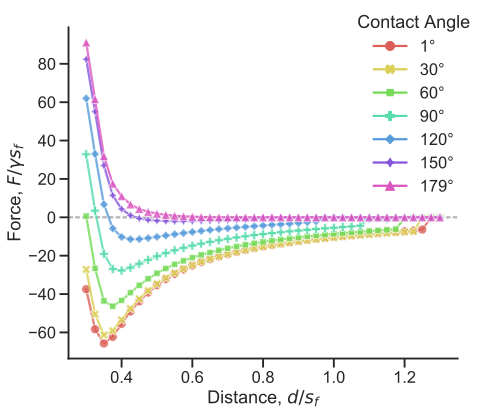
\includegraphics[scale=0.5]{Figure4a-Single_bridge_fd}

\subcaption{Force-distance curves}%
\end{minipage}\hfill{}%
\begin{minipage}[t]{0.5\columnwidth}%
\includegraphics[scale=0.5]{Figure4b-Single_bridge_force_contribution}

\subcaption{Force contributions}%
\end{minipage}\caption{\label{fig:Single-bridge}Normalized capillary force of a single liquid
bridge in contact with a substrate and pinned to a circular perimeter
on top. Fluid size parameter, $\phi_{f}=2$. Negative force values
represents attraction. a) Force-distance curves are shown for different
contact angles of the liquid with the substrate. b) Adhesion force,
calculated from the minima of the corresponding force-distance curve,
is plotted as a function of contact angle with the substrate, together
with its Laplace and surface tension components (equation \ref{eq:f_bridge}).
Simulation snapshots of the liquid meniscus corresponding to angles
6\textdegree{} and 150\textdegree{} are depicted.}
\end{figure}

The force-distance curves show a general trend of being repulsive
at small distances (Figure \ref{fig:Single-bridge}a). This is a result
of the pinned contact line on the top. A limited volume is available
for the liquid to occupy when the gap distance is small, causing the
meniscus shape to bulge outwards near the pinned contact line. This
creates a net positive curvature, resulting in a positive Laplace
pressure and thus repulsion.

\subsubsection{Capillary Bridge Model: Effect of the substrate\label{subsec:Capillary-Bridge-Model:}}

The normalized force-distance curves of a hairy pad system on a hydrophilic
and hydrophobic substrate are predicted based on the capillary bridge
model and compared for the different contact types (Figure \ref{fig:Effect-of-substrate}).
The forces in each case are calculated from equations (\ref{eq:f_air/water})
and (\ref{eq:f_bubble}) for fixed geometric and interfacial properties
(Table \ref{tab:Model-parameters}). 

On the hydrophilic substrate ($\theta_{wa}=24\lyxmathsym{\textdegree}$),
contact\emph{ in air} shows the highest adhesion. \emph{Underwater:
no bubble} shows close to no adhesion while \emph{underwater: bubble}
shows moderate adhesion. In contrast, for a hydrophobic substrate
($\theta_{wa}=120\lyxmathsym{\textdegree}$), the highest adhesion
is seen for \emph{underwater: no bubble}, much larger than \emph{in
air}. Even \emph{underwater: bubble} has slightly higher adhesion
than \emph{in air}. Note that the contact area is fixed by keeping
the area fraction and $D_{p}/D_{h}$ constant. All curves correspond
to the same total hair contact area. Thus, the above mentioned effects
are attributed solely to how the the capillary force changes in each
scenario.

On a hydrophilic substrate, the contact angle of the oily adhesive
fluid is 6\textdegree , when surrounded by air (Table \ref{tab:Model-parameters})
and 150\textdegree , when surrounded by water (equation (\ref{eq:theta_fw})).
This results in the meniscus shape to have a net negative and slightly
positive curvatures, respectively, resulting in strong adhesion in
air and poor adhesion underwater. On a hydrophobic substrate however,
the contact angles of the fluid in air and water are 50\textdegree{}
and 1\textdegree , respectively. In both cases, the contact angles
are low, resulting in strong adhesion in both media. Additionally,
the interfacial tension of the oily fluid underwater ($\gamma_{fw}$)
is twice that of in air ($\gamma_{fa}$). Thus, we see a higher capillary
adhesion for the \emph{underwater: no bubble} case when compared to
\emph{in air} (Figure \ref{fig:Oil-contact-images}).

\begin{figure}[H]
\centering{}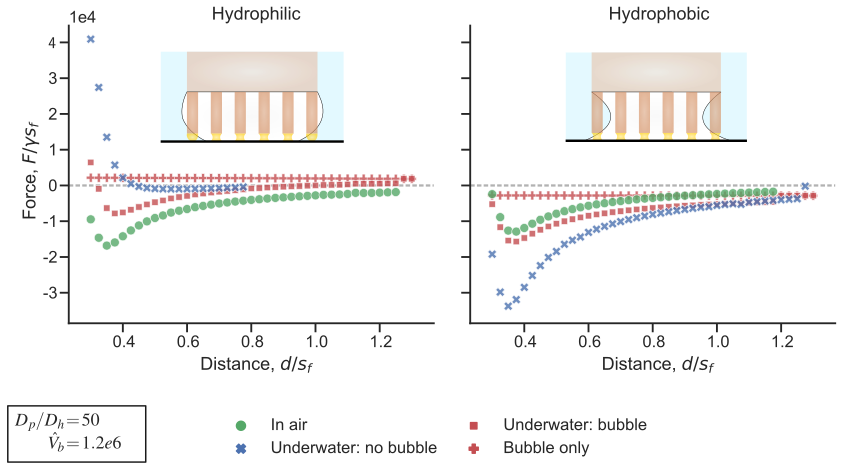
\includegraphics{Figure5-Model_effect_of_substrate}\caption{\label{fig:Effect-of-substrate}Theoretical force-distance curves
of a hairy pad system on a hydrophilic and hydrophobic substrate in
air and underwater conditions. A negative force value represents attraction.
Normalized forces are calculated from the capillary bridge model,
with model parameters listed in Table \ref{tab:Model-parameters}.
The bubble's contribution to the net force for an \emph{underwater:
bubble} contact is denoted by plus symbols. Insets represent the \emph{underwater:
bubble }contact for each substrate.}
\end{figure}

The net force in the \emph{underwater: bubble} case mainly depends
on the proportion of hairs inside and outside the bubble (equation
(\ref{eq:f_bubble})). For the given bubble volume, only part of the
hairs are inside the bubble for the hydrophilic substrate, while,
all the hairs are inside the bubble for the hydrophobic substrate.
Therefore, the force curve lies between \emph{in air} and \emph{underwater:
no bubble} cases for a hydrophilic substrate, and closely follows
the \emph{in air} case for a hydrophobic substrate.

The contribution of the capillary force due to the bubble itself is
negligible for both substrates (Figure \ref{fig:Effect-of-substrate}).
Its contribution even is slightly repulsive on the hydrophilic substrate
due to the positive curvature of the bubble, and slightly attractive
on the hydrophobic substrate due to its negative curvature. This small
contribution is manifested by the slightly higher adhesion for \emph{underwater:
bubble} relative to \emph{in air} for the hydrophobic substrate, since
all hairs are within the bubble in this case.

\subsubsection{Capillary Bridge Model: Effect of bubble volume}

The effect of varying bubble volume, $\hat{V}_{b}$, on the net adhesion
force of the \emph{underwater: bubble} case are compared for hydrophilic
and hydrophobic substrates (Figure \ref{fig:Effect-of-bubble}). From
previous section, we know that on the hydrophilic substrate, fluid
bridges outside the bubble show poor adhesion due to the positive
curvature of their meniscus. Thus, decreasing $\hat{V}_{b}$ decreases
the adhesion force due to a larger proportion of hairs being outside
the bubble. In contrast, on the hydrophobic substrate, fluid bridges
outside the bubble show higher capillary forces, due to its low contact
angle and high interfacial tension in water. Thus, adhesion force
increases for a hydrophobic substrate as the bubble size decreases. 

\begin{figure}[H]
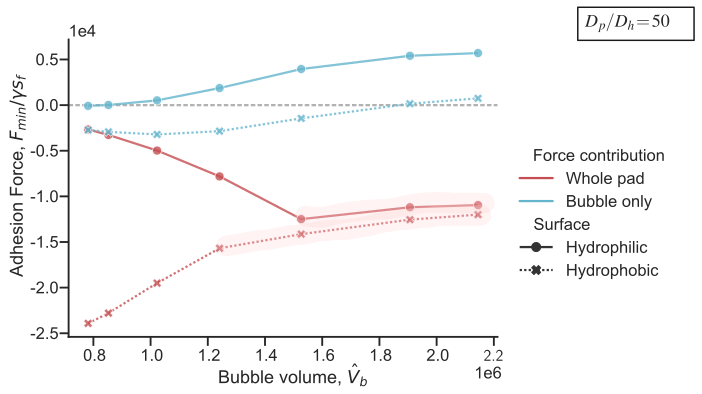
\includegraphics{Figure7-Model_effect_of_bubble_volume}\caption{\label{fig:Effect-of-bubble}Normalized adhesion force of a hairy
pad system as a function of bubble volume, $\hat{V}_{b}$, for the
\emph{underwater: bubble} contact type. Adhesion forces are calculated
from the minima of the respective force-distance curves. Negative
force value represents attraction. Pad to hair diameter ratio ($D_{p}/D_{h}$)
is kept fixed. Highlighted regions represent entrapment of all hairs
within the bubble.}
\end{figure}
The contribution of the bubble to the net adhesion force is small
regardless of its volume, when compared to the whole pad. We see that
a smaller $\hat{V}_{b}$ results in increased attraction by the bubble
on both types of substrates. For larger values of $\hat{V}_{b}$,
the force trend for the whole pad mostly follows that of the bubble,
because the bubble in this case is big enough to entrap all the hairs
inside it. Thus, the force contribution due to the fluid bridges remain
unchanged, and only the bubble's contribution drives the slight variation
in the pad's adhesion at high $\hat{V}_{b}$. Once the bubble is small
enough such that part of the fluid bridges start making contact in
water, the force trend changes, with a steep decrease (increase) in
adhesion force on hydrophilic (hydrophobic) substrate as the volume
decreases.

\subsubsection{Capillary Bridge Model: Effect of hair diameter }

The effect of changing hair diameter, $D_{h}$, to the net adhesion
force is compared for hydrophilic and hydrophobic substrates (Figure
\ref{fig:Effect-of-hair}). Here, the pad diameter, total hair contact
area and bubble volume are constant since $D_{p}$, $\alpha$ and
$\hat{V}_{b}$ are kept fixed. The radius corresponding to the fluid
volume is assumed to scale proportional to the hair diameter and is
fixed ($\phi_{f}=2$).

Adhesion force increases with decreasing $D_{h}$ for both hydrophilic
and hydrophobic substrates in all contact types. This is consistent
with the ``contact splitting'' theory, which predicts higher adhesion
when the contact is split into many small contact points\cite{RN24}.
Reducing the hair diameter results in two competing effects: 1) capillary
force due to a single fluid bridge decreases due to its smaller size
and ``self-similar'' scaling assumption ($f\sim D_{h}$), which
decreases the net force, and 2) total number of fluid bridges increases
since the total hair contact area is assumed to be fixed ($N\sim1/D_{h}^{2}$),
which increases the net force. The second effect dominates, resulting
in a higher adhesion force as $D_{h}$ decreases. 

\begin{figure}[H]
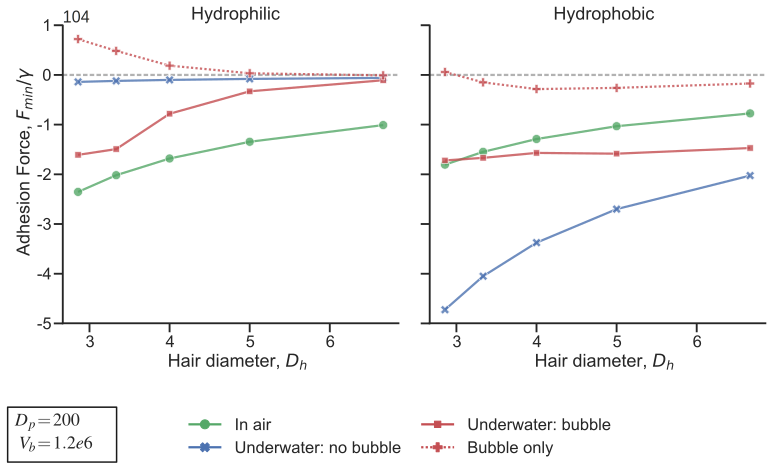
\includegraphics[scale=0.5]{Figure6-Model_effect_of_hair_size}\caption{\label{fig:Effect-of-hair}Normalized adhesion force of a hairy pad
system on a hydrophilic and hydrophobic substrate as a function of
hair diameter, $D_{h}$. Volume of each fluid bridge, $V_{f}$, scales
relative to $D_{h}$ based on the parameter $\phi_{f}=2$. Adhesion
forces are calculated from the minima of the respective force-distance
curves, based on the capillary bridge model. A negative value represents
attraction. The bubble's contribution to the net force for an \emph{underwater:
bubble} contact is denoted by plus symbols. Pad diameter and bubble
volume are kept fixed. All lengths are scaled relative to $D_{p}$.}
\end{figure}

Similar to the trend in Figure \ref{fig:Effect-of-substrate}, contact
\emph{in air} shows the highest adhesion force on a hydrophilic substrate
for the given range of hair diameters, while on a hydrophobic substrate,
\emph{underwater: no bubble} shows highest adhesion. \emph{Underwater:
bubble} contact shows intermediate adhesion between \emph{in air}
and \emph{underwater: no bubble} contact types.

The bubble's contribution gets repulsive as hair diameter decreases
for both substrates (Figure \ref{fig:Effect-of-hair}). Since the
aspect ratio $L/D_{h}$ is fixed (Table \ref{tab:Model-parameters}),
decreasing the hair diameter also decreases its length. Since the
bubble's volume is kept constant, it will then have a lesser space
available to occupy between the pad and the substrate, This results
in it bulging outwards near the pinned contact line on the top. Thus,
the bubble's contribution gets repulsive as hair diameter decreases.

\section{Discussion}

Our experiments demonstrate, for the first time, that the ladybug
beetle can attach underwater to a hydrophobic substrate even without
a bubble trapped around its hairs. A previous study\cite{RN87} had
hypothesized that a bubble is necessary for underwater attachment
in beetles. This is, however, only true for hydrophilic substrates,
where a trapped bubble can facilitate underwater adhesion due to the
hairs making contact in a dewetted environment. For a hydrophobic
substrate, the adhesion is similar regardless of whether the contact
occurs in air or underwater conditions, with or without a trapped
bubble. Our theoretical calculations further show that the bubble
by itself has a negligible capillary contribution to the net underwater
adhesion of the pad. Direct force measurement of a single similarly
sized bubble making contact with a hydrophobic substrate shows a maximum
adhesion less than 50 \textgreek{m}N, which further validates that
the bubble's contribution is insignificant (\ref{subsec:Capillary-force-due}).

Predictions of the ladybug's adhesion from the capillary bridge model
follow our experimental results (Figure \ref{fig:Effect-of-contact}).
In underwater conditions without a trapped bubble, adhesion on a hydrophobic
substrate is significantly larger than on a hydrophilic substrate.
This is explained by the different oil interfacial tension and contact
angles with the substrates in air and underwater, which determines
the capillary adhesive force in each case (Figure \ref{fig:Oil-contact-images}).
However, the experiments don't show the predicted $\sim$ 2.6 times
increase in underwater adhesion relative to that in air on the hydrophobic
PFOTS surface. This discrepancy could be due to our assumptions of
the oily fluid's interfacial properties. If we choose $\gamma_{fa}$=30
mN/m and $\gamma_{fw}$=40 mN/m, the corresponding increase in adhesion
will be $\sim$ 1.7, closer to our experimental value of $\sim$ 1.
The resulting change in $\theta_{fa}$ and $\theta_{fw}$ will further
decrease this number. Direct measurement of the fluid's interfacial
properties is thus essential to better predict the insect's adhesion,
and will be a subject of future study. Further, due to surface inhomogeneities,
not all the hairs might be able to completely drain the interfacial
water layer, in order for the adhesive fluid to make a direct contact
with the substrate. This can further reduce underwater adhesion, in
comparison to our theoretical predictions which assumes a perfect
contact.

\begin{figure}[H]
\includegraphics{Figure-8-contact_angle_schematic}\caption{\label{fig:Oil-contact-images}Simulation snapshots of oil capillary
meniscus in contact with glass and PFOTS in air and underwater conditions.
The corresponding interfacial tension, \textgreek{g}, and contact
angle, \ensuremath{\theta}, used to predict the ladybug's adhesion
are labeled for each case.}
\end{figure}

In the model, we assume that all the hairs detach simultaneously to
give a theoretical maximum achievable adhesion force. In our experiments,
however, the pad always makes contact with the substrate at a random
orientation, which is difficult to control precisely. During detachment,
the pad typically peels off from its proximal to distal end rather
than detach simultaneously. Our model also assumes the hairs to be
of similar geometry, unlike the beetle's pad which has a distribution
of flat or pointed tipped hairs. Thus, it's not surprising that the
model overestimates the adhesion forces. The predictions are however
in the same order of magnitude as experiments, and the qualitative
trend is consistent for both hydrophilic and hydrophobic substrates
in air and underwater.

Our study provides further validation that capillary forces by the
adhesive fluid control the insect's adhesion and van der Waals contribution,
if any, must be negligible. Further, the capillary forces can even
enable insect attachment underwater depending on the substrate chemistry.
When underwater, without a trapped bubble, the pad adheres strongly
to a hydrophobic substrate, but poorly to a hydrophilic substrate,
even though it shows similarly strong adhesion to both substrates
in air. This behavior can only be explained by capillary forces. Our
preliminary FDMS results further provides validation to our assumption
that the adhesive fluid can form capillary bridges with the substrate
in water, instead of getting washed away (Table \ref{tab:Molecular-distribution-of}).

The findings can also be extended to other animals relying on oily
secretions for adhesion. Ants, for example, show similar adhesion
on hydrophobic substrates under wet and dry conditions\cite{RN213},
similar to what we see in a ladybug. Recent adhesion experiments on
geckos reveal that they can attach well to fluoropolymer substrates
underwater while they show little adhesion to the same substrate in
air\cite{RN199,RN15}. Geckos are thought to rely on van der Waals
forces via dry contact with the substrate \cite{RN202}, although
recent observations of phospholipid footprints left behind walking
geckos \cite{RN205} could change that picture. Since geckos adhere
poorly to PTFE (surface energy \textasciitilde{} 20 mN/m) one can
speculate that the phospholipid material has a higher surface energy,
and consequently makes a higher contact angle with PTFE in air. Let
us assume the phosopholipid substance to be a fluid similar to oil
with $\gamma_{fa}$= 30 mN/m and $\gamma_{fw}$= 42 mN/m such that
its contact angle with PTFE is 80\textdegree . Equation \ref{eq:theta_fw}
then gives us an underwater contact angle of 70\textdegree{} for the
phospholipid fluid. Thus, on a PTFE surface, the capillary bridge
model can predict a higher adhesion underwater than in air due to
its lower contact angle and higher interfacial energy underwater.
Based on similar assumptions, we predict the net adhesion force for
the gecko on different substrates (Figure \ref{fig:Comparison-with-model}).
The adhesion force predictions are in good qualitative agreement with
the whole animal experimental shear force values reported for the
gecko, with the trend of higher adhesion in air than underwater for
glass, similar adhesion in air and underwater for PMMA/OTS-SAM and
lower adhesion in air than underwater for PTFE. We, thus, propose
that the underwater experiments performed on geckos \cite{RN199,RN15}
indicate a capillary contribution to gecko adhesion. We suggest performing
single seta adhesion force tests similar to Autumn et. al. \cite{RN202}
using a hydrophilic and fluorinated probe in air and underwater conditions
to validate the role of capillary contributions to gecko adhesion.

\begin{figure}[H]
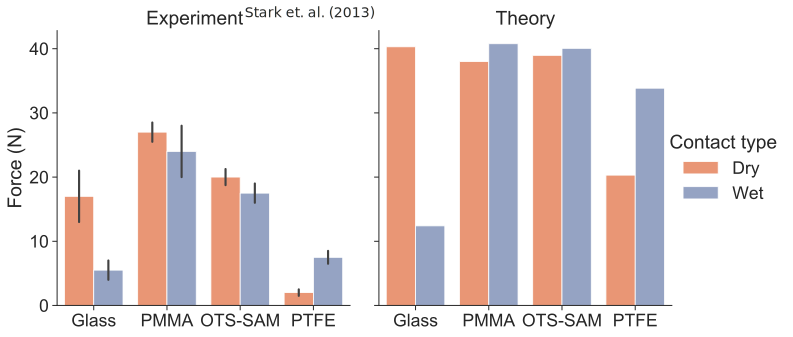
\includegraphics{Figure-9-Gecko_comparison}\caption{\label{fig:Comparison-with-model}Whole animal adhesion force of geckos
on various substrates. Experimental shear adhesion values are reproduced
from Stark et. al. \cite{RN15}. Normal adhesion forces for each gecko
toe are theoretically estimated from the capillary bridge model, with
hair diameter = 400 nm, toe diameter = 4 mm, adhesive fluid volume
= 4.19x10\protect\textsuperscript{-3} fL and 10\% hair coverage.
\textquotedblleft\emph{Underwater: no bubble}\textquotedblright{}
type contact is assumed for the \textquotedblleft Wet\textquotedblright{}
case. Net adhesion force is calculated by assuming 5 toes on each
leg and 4 legs in total on a gecko. Interfacial tension of the phospholipid
layer (PL) in air and water are assumed to be 30 mN/m and 42 mN/m
respectively. PL contact angles with glass, PMMA, OTS-SAM and PTFE
are assumed to be 6\textdegree , 10\textdegree , 20\textdegree{} and
80\textdegree{} respectively. The corresponding water contact angles
are 50\textdegree , 85\textdegree , 94\textdegree{} and 97\textdegree{}
respectively, as reported in Stark et. al. \cite{RN15}.}
\end{figure}

We have so far limited our analysis to only smooth substrates. Insects
in the real world, however, interact with rough substrates very often.
Previous studies \cite{RN136} have shown that substrate roughness
is a more dominant parameter than substrate chemistry in controlling
insect adhesion. Future work will explore how roughness can impact
the net capillary force. Our study can have potential applications
in the design of bio-inspired materials to achieve underwater adhesion
via capillary bridges. Bubble can possibly be used to control underwater
adhesion by changing the relative proportion of the arrays inside
and outside the bubble. A suitable choice of adhesive fluid can be
made tailored to the substrate and environment of application to achieve
optimal adhesion performance.

\section{Conclusions}

Our study illustrates that the ladybug beetle relies primarily on
its oily fluid secretion to achieve adhesion in both air and underwater
conditions. The beetle can attach underwater on a hydrophobic substrate
even without a trapped air bubble within its hairy pad, although it
loses this ability on a hydrophilic substrate. This is explained theoretically
by the different contact angle and interfacial tension of the adhesive
fluid in air and underwater conditions. Further, the bubble itself
has a negligible capillary contribution to the total force. The trapped
bubble can promote adhesion only on a hydrophilic substrate by providing
an air medium to the adhesive fluid bridges inside it. Oil wettability,
thus, primarily controls the insect's adhesion in any given condition.
A similar argument also explains previously reported underwater measurements
in geckos \cite{RN15}, which highlights the possibility of capillary
contributions to gecko adhesion. Future studies should characterize
the fluid secretion's interfacial properties with a particular substrate
to better understand the nature of the animal's adhesion.

\section{Acknowledgement}

We are grateful to Eduard Arzt and Ren\textcyr{\`\cyre} Hensel for
fruitful discussions. This work was funded by \emph{Deutsche Forschungsgemeinschaft}
(Grant number: PI 1351/2-1). 

\appendix

\section{Appendix}

\subsection{Simulation method: Single capillary bridge \label{subsec:Simulation-Method}}

\setcounter{figure}{0} \renewcommand{\thefigure}{A.\arabic{figure}} 
\setcounter{equation}{0} \renewcommand{\theequation}{A.\arabic{equation}} Capillary
force due to a single adhesive fluid or bubble meniscus (termed ``capillary
bridge'') is calculated by performing simulations in Surface Evolver
\cite{RN206}, similar to the method described by De Souza et. al.\cite{RN93}.
A simple cubic geometry, mimicking the capillary bridge, of constant
volume, $V$, is defined as the initial condition with an interfacial
tension, $\gamma$, with the surrounding medium. Interfacial tension
of the capillary bridge with the substrate is given by $\gamma\cos\theta$,
where $\theta$ is the corresponding contact angle inside the bridge.
For the case of a bubble meniscus, $\theta$ is defined w.r.t. the
surrounding water, since $\theta$ can also directly characterize
the substrate wettability. The capillary bridge spans a gap distance
$d$ between the top face and the substrate. The boundary conditions
are set corresponding to a pinned contact line of diameter $D$ on
the top face and constant interfacial tension with the substrate on
the bottom. All lengths are normalized relative to length $s=\left(3V/4\pi\right)^{1/3}$.
An appropriate geometry refinement routine is chosen to evolve the
capillary bridge shape to its minimum energy state. The normalized
total capillary force, $\hat{f}=f/\gamma s$, is the sum of the Laplace
pressure and surface tension contributions , where:

\begin{equation}
f=f_{laplace}+f_{surface\,tension}=\varDelta P_{laplace}A_{_{bottom}}+2\pi R_{bottom}\gamma\sin\theta\label{eq:f_bridge}
\end{equation}

Here, $\varDelta P_{laplace}$ is the Laplace pressure of the equilibrium
capillary bridge, $A_{bottom}$ is the contact area of the capillary
bridge with the substrate at bottom and $R_{bottom}$ is the corresponding
radius of contact, all obtained from the simulation output for the
equilibrium surface.

The gap distance $d$ is varied stepwise and the capillary force is
calculated each time to obtain force-distance curves for a particular
choice of $D$ and $\theta$. 

\subsection{Single capillary bridge: Effect of volume}

Surface Evolver simulation results showing the effect of volume on
the maximum capillary force of a single fluid bridge. Since the fluid
is pinned at the top to the same diameter, D, a smaller volume would
result in high interfacial curvatures, which increases the capillary
force due to the negative Laplace pressure. In this case, small contact
angles lead to a greater increase in adhesion.

\begin{figure}[H]

\begin{centering}
\includegraphics{FigureS2-Effect_of_fluid_volume}\caption{Normalized maximum capillary force for a single bridge as a function
of fluid volume}
\par\end{centering}
\end{figure}


\subsection{Capillary Bridge Model: Effect of hair diameter at constant fluid
volume}

Here, instead of scaling the fluid volume relative to the hair diameter,
we now assume a fixed total fluid volume distributed equally among
the $N$ hairs. Total fluid volume, $V_{total}=NV_{f}=2000$. Hair
diameter is varied while keeping the total hair contact area constant.
Length is in arbitrary units. Forces increase at a much smaller rate
on decreasing diameter when compared to the case with self-similar
scaling of fluid volume (Figure \ref{fig:Effect-of-hair}).

\begin{figure}[H]
\includegraphics{FigureS3-Effect_of_hair_size(constant_vol)}

\caption{Normalized adhesion force of hairy pad system on a hydrophilic and
hydrophobic substrate as a function of hair diameter ($D_{h}$), calculated
from the capillary bridge model. The total adhesive fluid volume is
fixed to 2000. Adhesion forces are calculated from minima of the respective
force-distance curves. Negative force value represents attraction.
The bubble's contribution to the net force for an \emph{underwater:
bubble} contact is denoted by plus symbols. Bubble volume and pad
diameter are kept fixed. All lengths are scaled relative to $D_{p}$.}
\end{figure}


\subsection{Capillary force due to a bubble\label{subsec:Capillary-force-due}}

Capillary force of a single bubble against a PFOTS surface are compared
for two different volumes. The volumes correspond to the expected
range in the case of the trapped bubble in a ladybug. Here, the bubble
is pinned to a micropatterned PDMS substrate on the top. The maximum
adhesion force of any of the bubble never exceeds 50 \textgreek{m}N,
significantly lower than the beetle's underwater adhesion to the same
substrate (> 400 \textgreek{m}N). Thus, the bubble's contribution
to adhesion in the ``\emph{underwater: bubble}'' contact of a ladybug's
pad should be negligible.

\begin{figure}[H]
\begin{centering}
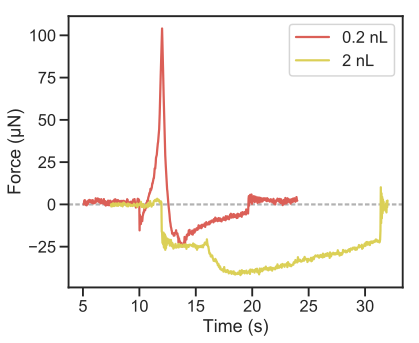
\includegraphics{FigureS4-Expt_bubble_force}\caption{Capillary force of the bubble}
\par\end{centering}
\end{figure}

\bibliography{references}

\end{document}
